% Appendix: UML diagrams drawn by analysis/phase1/uml_figures.py from the design in the code,
% and the state ownership and error handling the project asks to be defined explicitly.
\section{UML diagrams, state ownership and error handling}
\label{sec:uml}

This appendix adds to the diagrams in the body of the report. It shows the system from the views the body does not draw, using the names in the code, on the final build with the rotating-rounds shared log.

\subsection{Structure}

\begin{figure}[!htb]
\centering
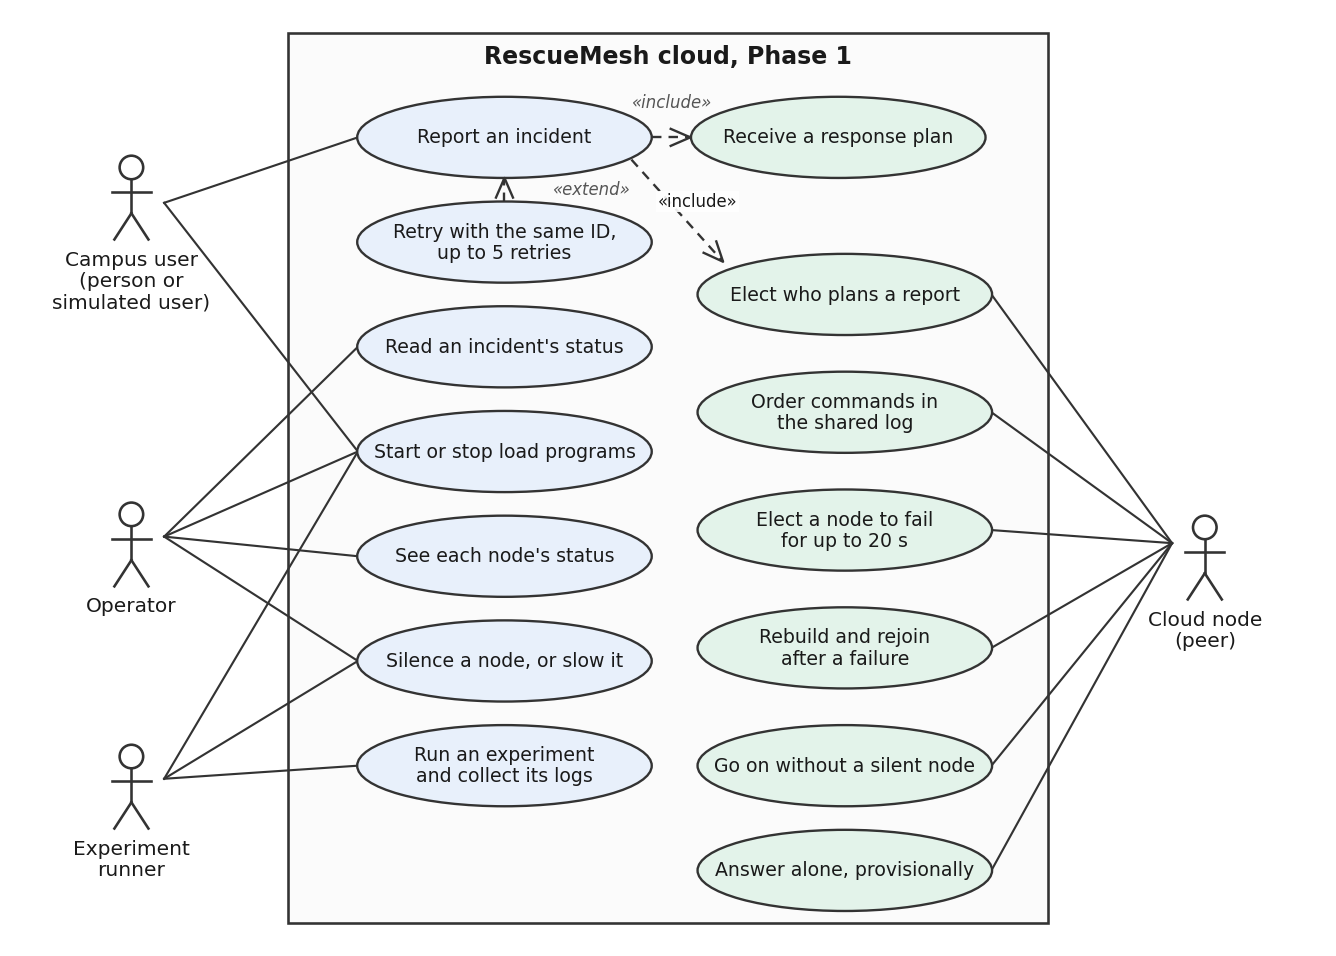
\includegraphics[width=0.86\linewidth]{figures/uml-use-cases.png}
\caption{UML use case diagram of the Phase 1 cloud. A dashed arrow marks an included or extending use case.}
\label{fig:uml-use-cases}
\end{figure}

\begin{figure}[!htb]
\centering
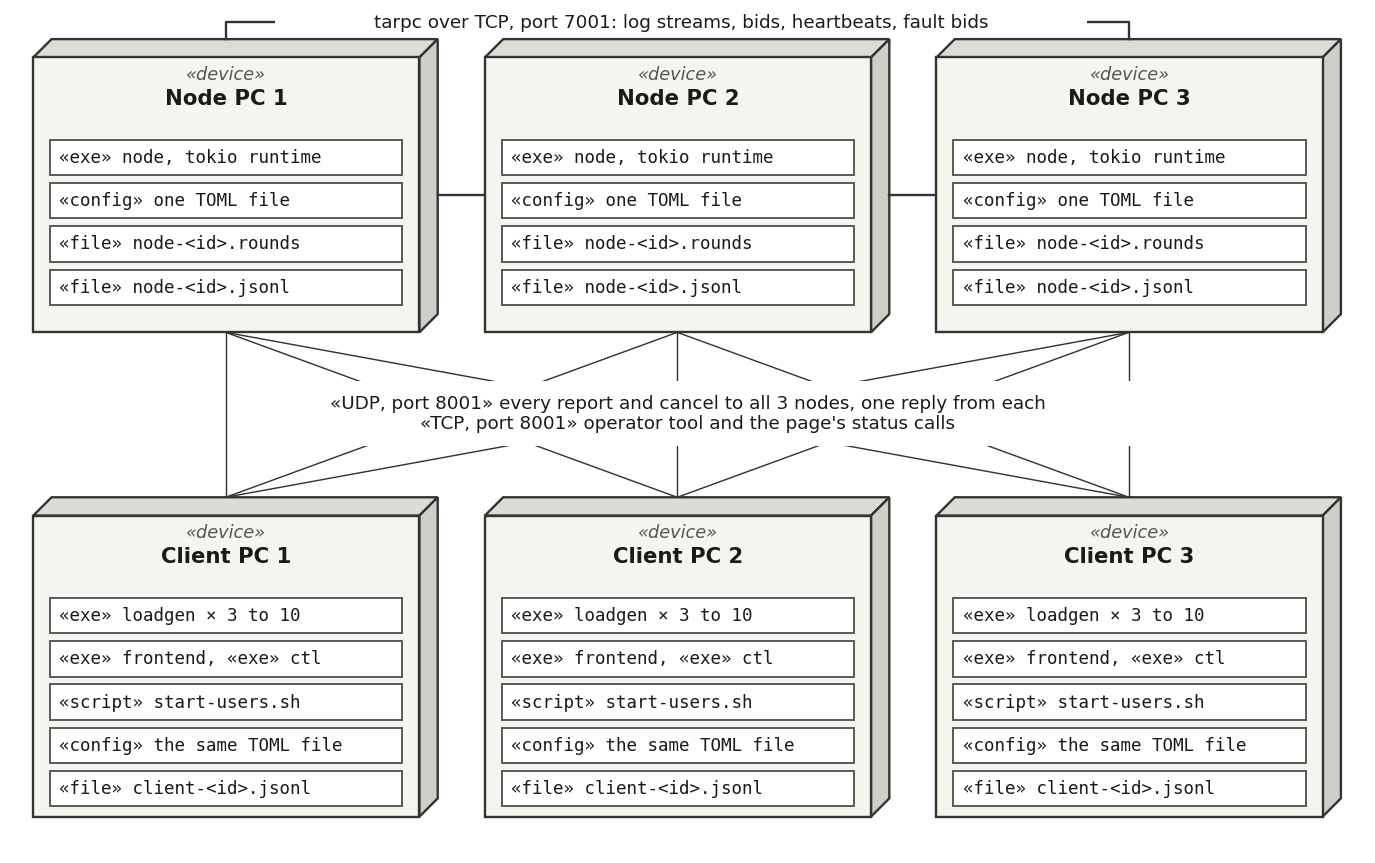
\includegraphics[width=0.92\linewidth]{figures/uml-deployment.png}
\caption{UML deployment diagram: the six PCs, what runs on each, and the paths between them.}
\label{fig:uml-deployment}
\end{figure}

\begin{figure}[!htb]
\centering
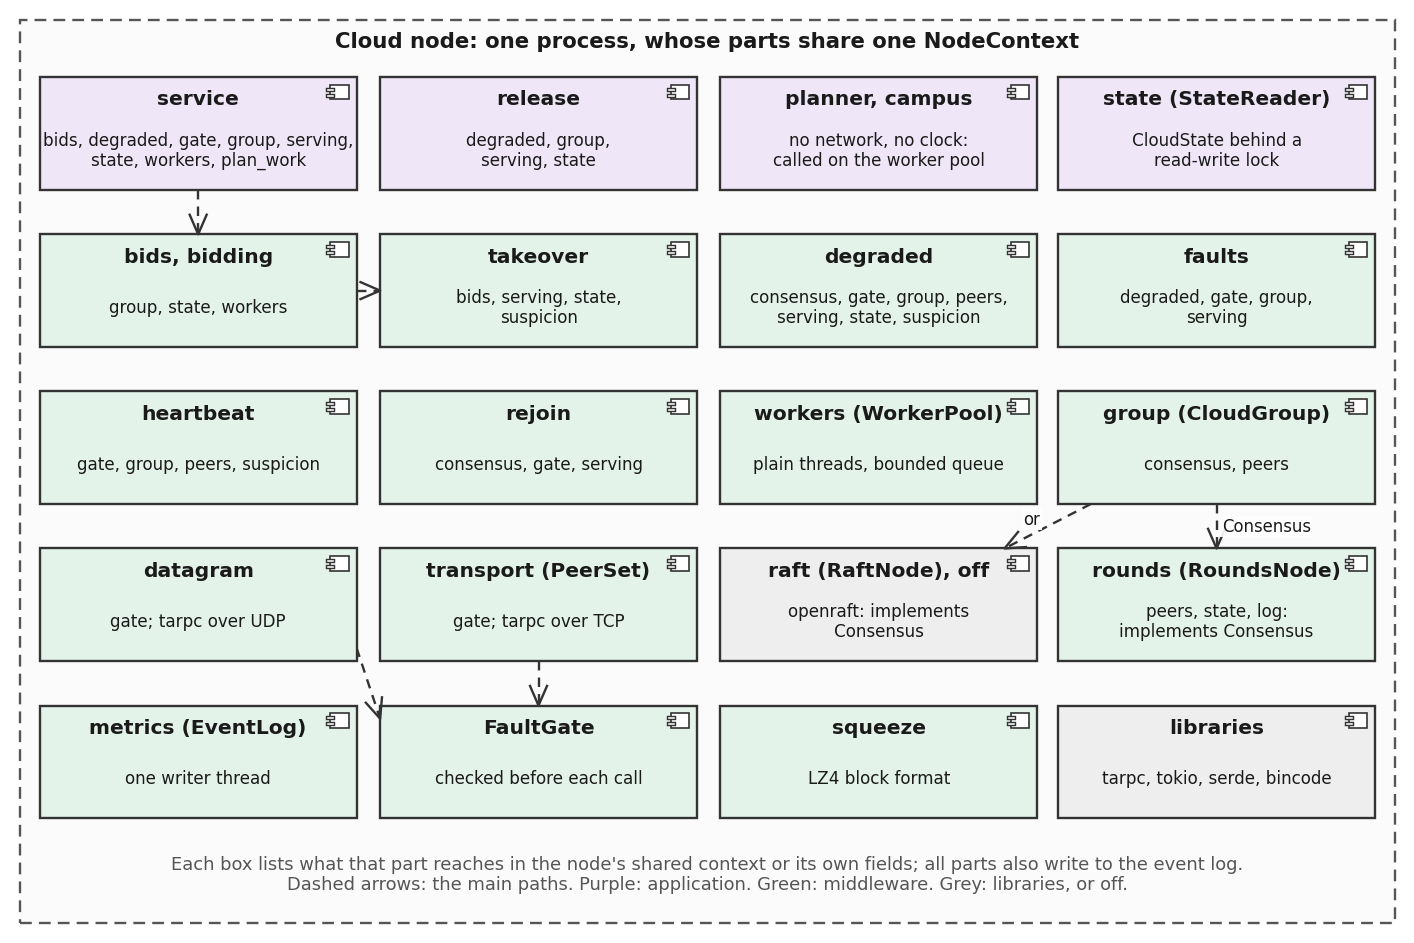
\includegraphics[width=\linewidth]{figures/uml-components.png}
\caption{UML component diagram of one cloud node.}
\label{fig:uml-components}
\end{figure}

\begin{figure}[!htb]
\centering
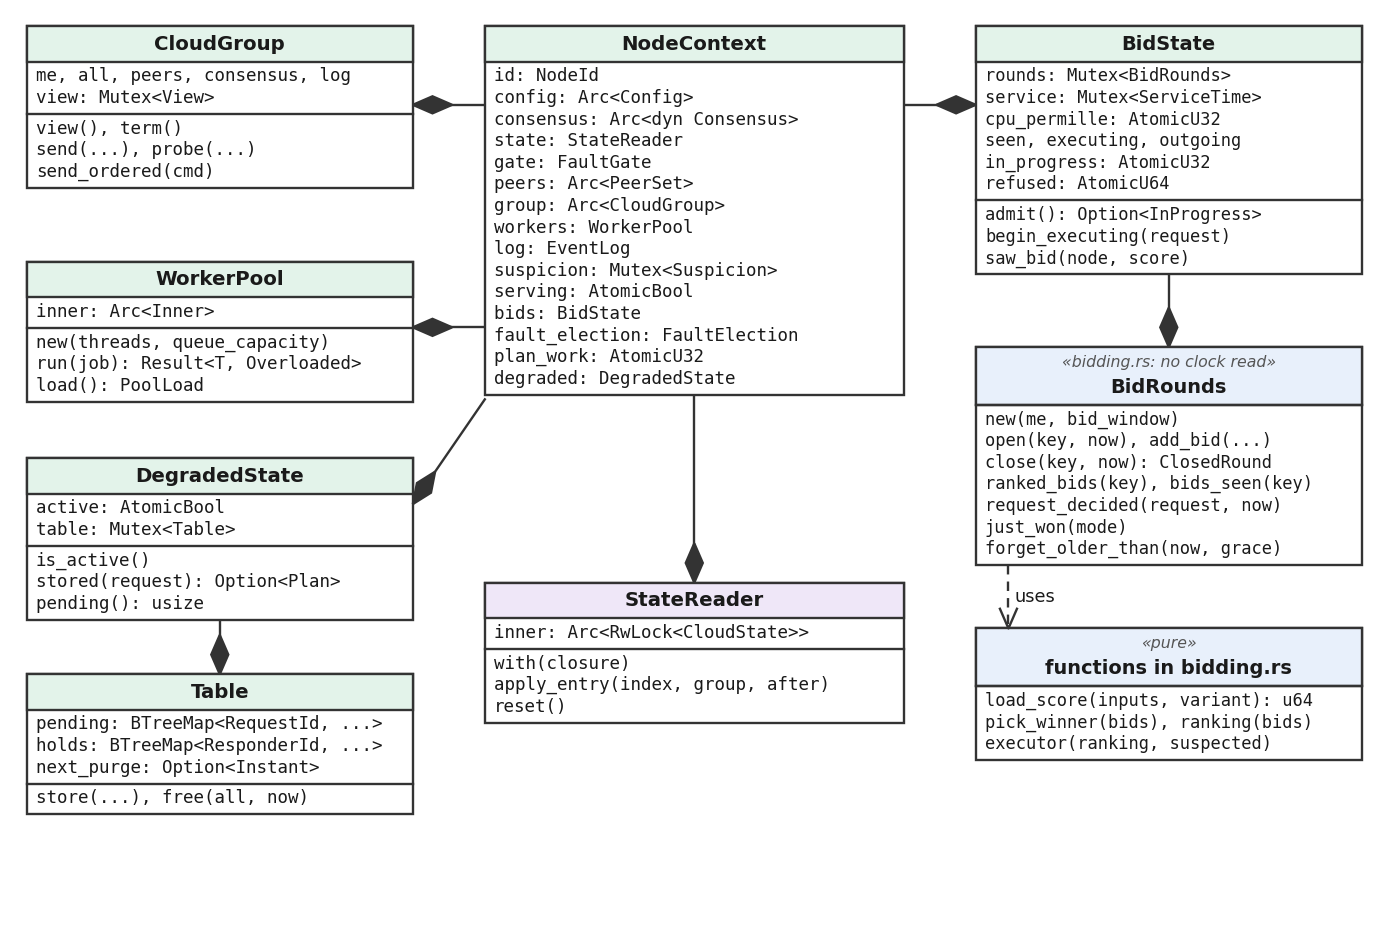
\includegraphics[width=0.92\linewidth]{figures/uml-class-node.png}
\caption{UML class diagram of a node's shared context and the parts it holds. A filled diamond means the whole owns the part.}
\label{fig:uml-class-node}
\end{figure}

\begin{figure}[!htb]
\centering
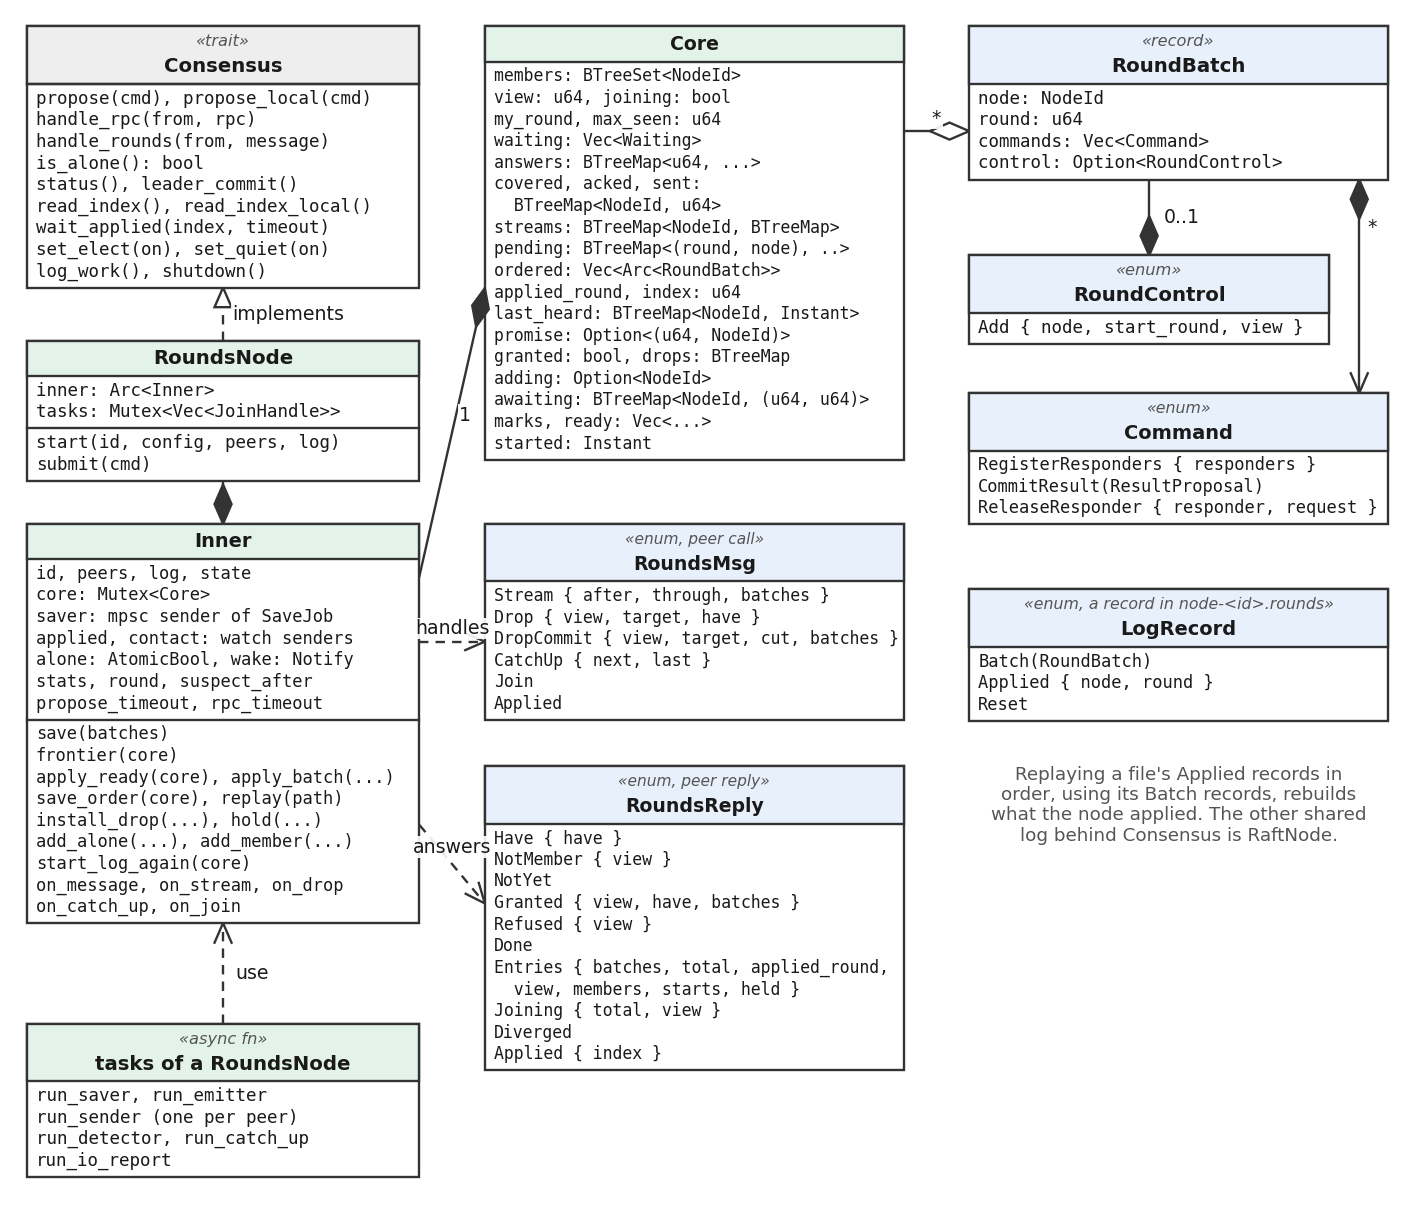
\includegraphics[width=\linewidth]{figures/uml-class-log.png}
\caption{UML class diagram of the shared log: its implementation of the interface, its state, its messages and its file records.}
\label{fig:uml-class-log}
\end{figure}

\begin{figure}[!htb]
\centering
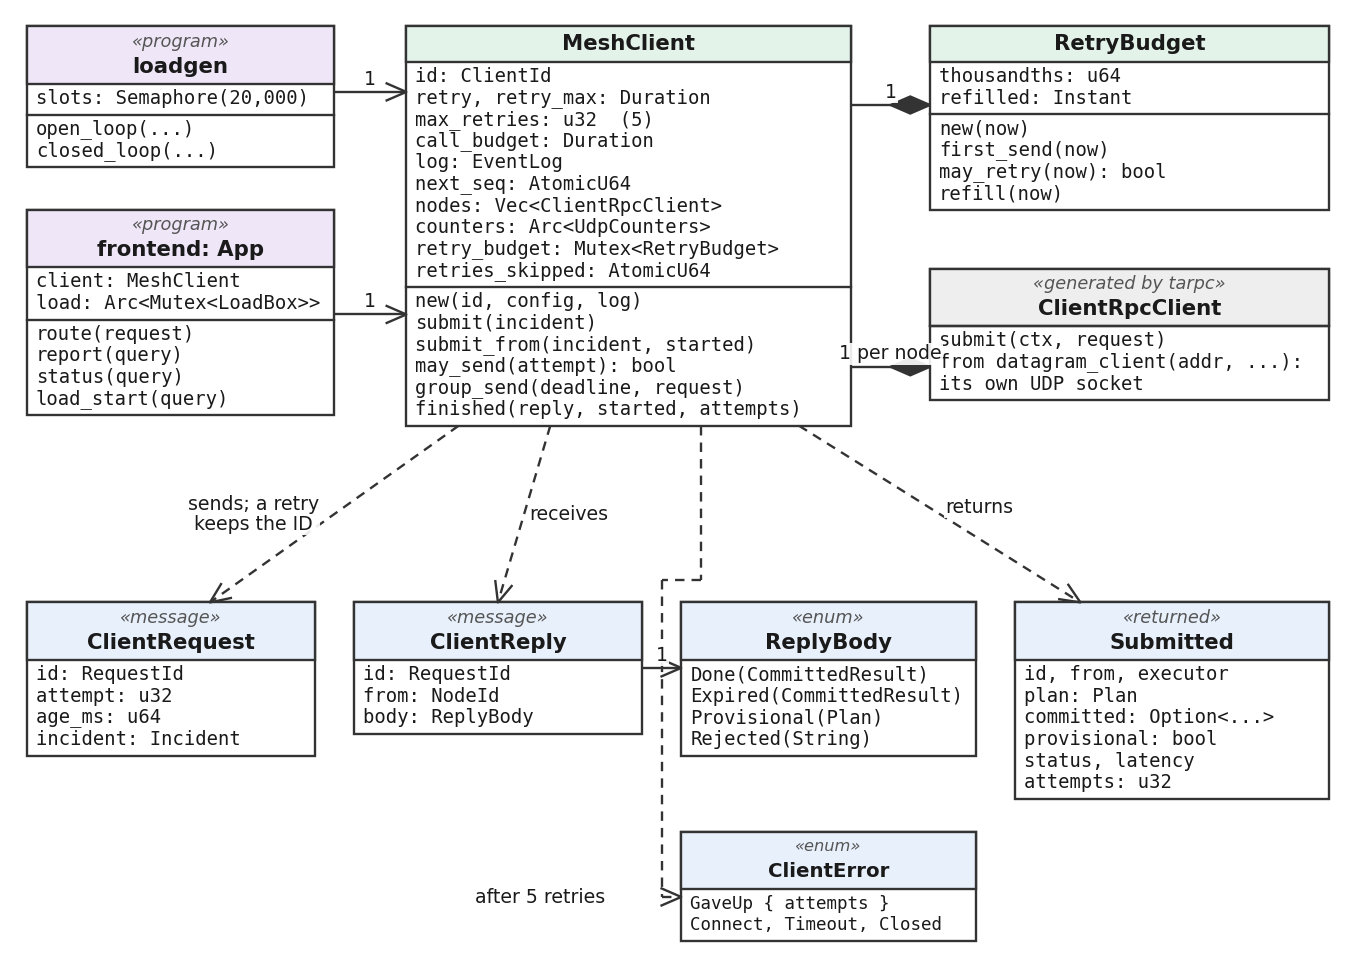
\includegraphics[width=0.92\linewidth]{figures/uml-class-client.png}
\caption{UML class diagram of the client side: the programs, the client middleware and its retry budget, and the messages.}
\label{fig:uml-class-client}
\end{figure}

\clearpage
\subsection{Behaviour}

\begin{figure}[!htb]
\centering
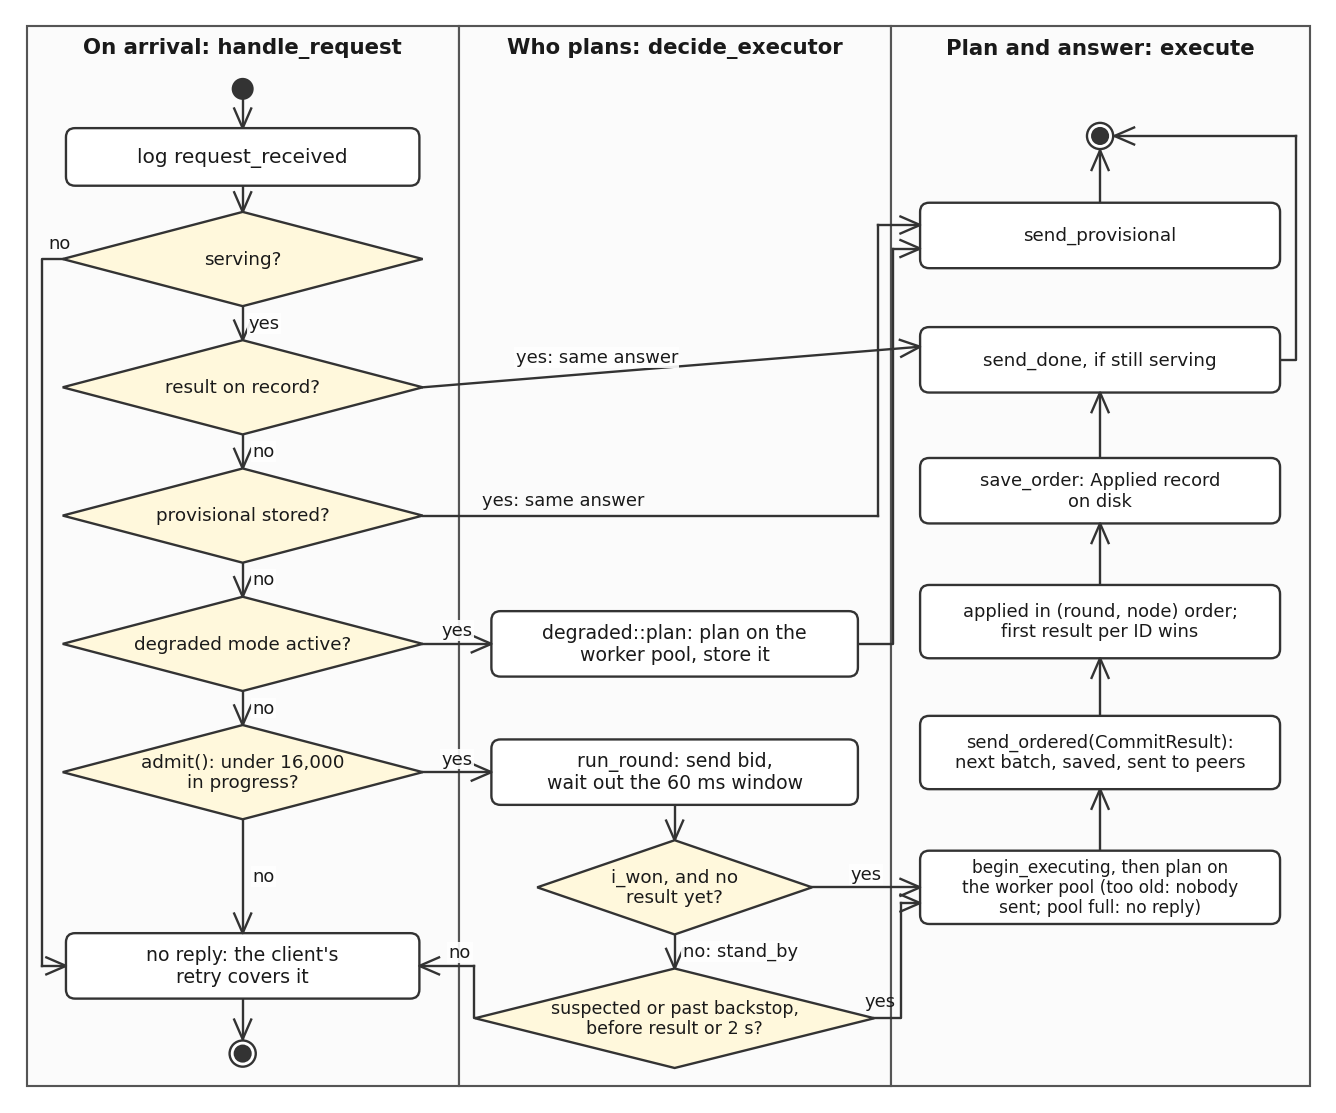
\includegraphics[width=0.95\linewidth]{figures/uml-activity.png}
\caption{UML activity diagram: what one node does with one report.}
\label{fig:uml-activity}
\end{figure}

\begin{figure}[!htb]
\centering
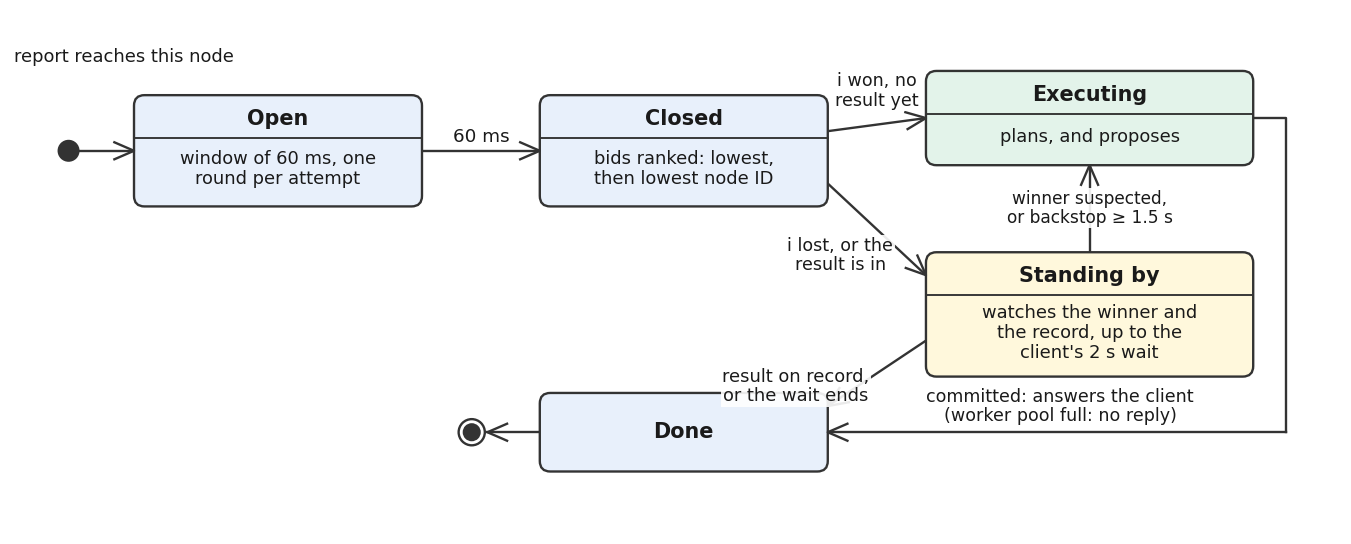
\includegraphics[width=0.86\linewidth]{figures/uml-state-bid.png}
\caption{UML state machine of one bidding round on one node.}
\label{fig:uml-state-bid}
\end{figure}

\begin{figure}[!htb]
\centering
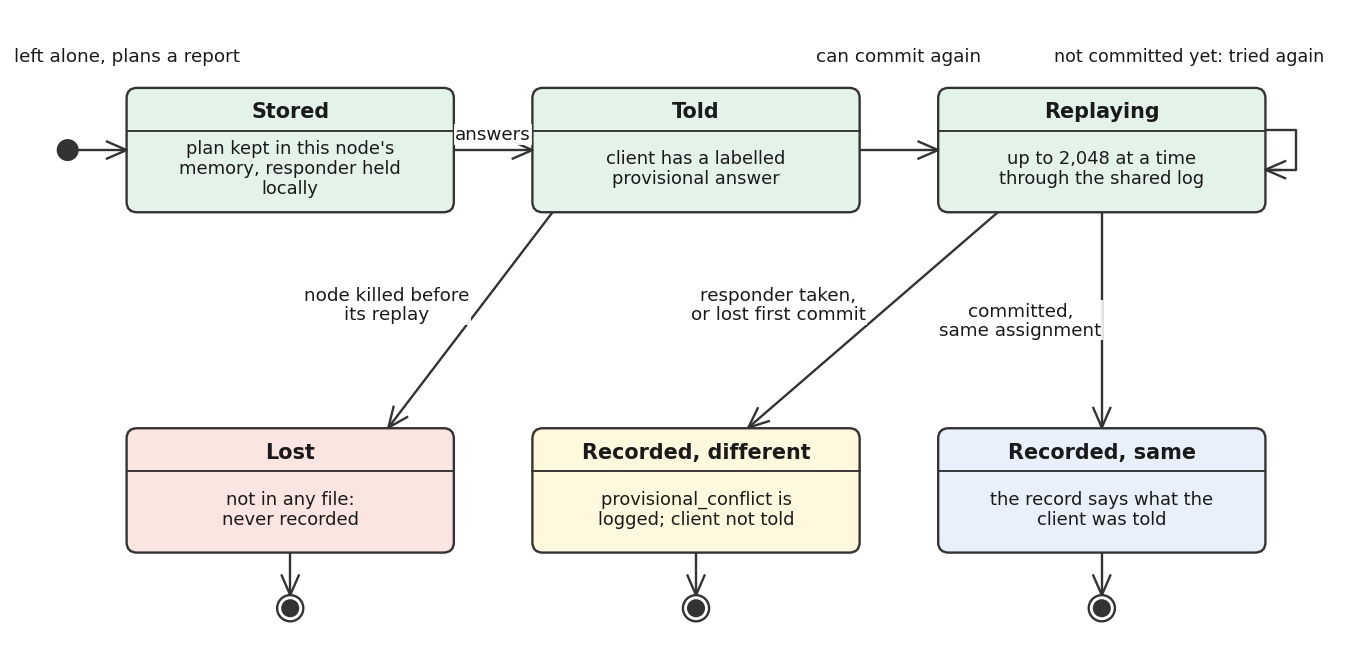
\includegraphics[width=0.86\linewidth]{figures/uml-state-provisional.png}
\caption{UML state machine of one provisional answer from a node left alone.}
\label{fig:uml-state-provisional}
\end{figure}

\begin{figure}[!htb]
\centering
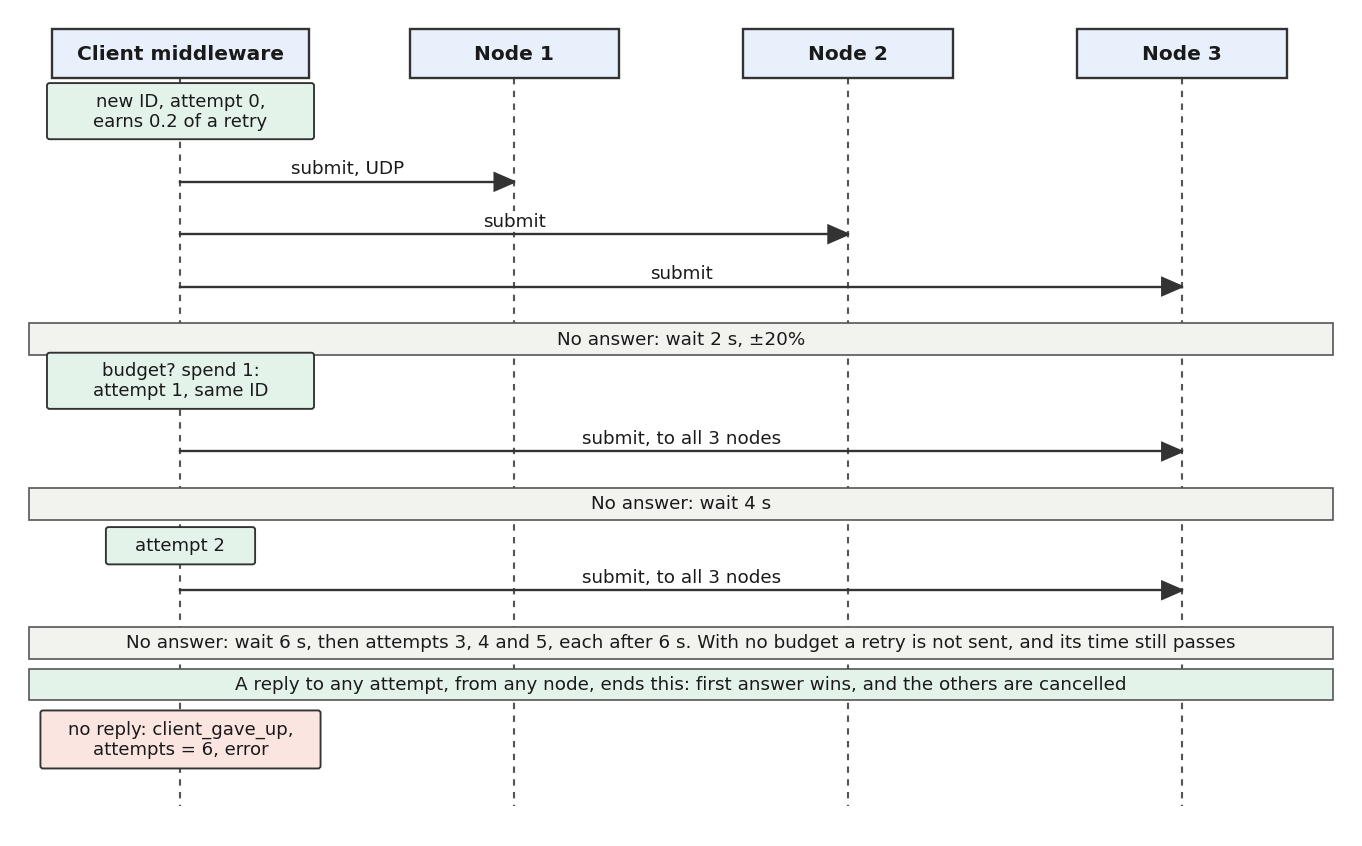
\includegraphics[width=0.88\linewidth]{figures/uml-seq-retries.png}
\caption{UML sequence diagram: a client's retries with every node off, 5 retries and then an error.}
\label{fig:uml-seq-retries}
\end{figure}

\begin{figure}[!htb]
\centering
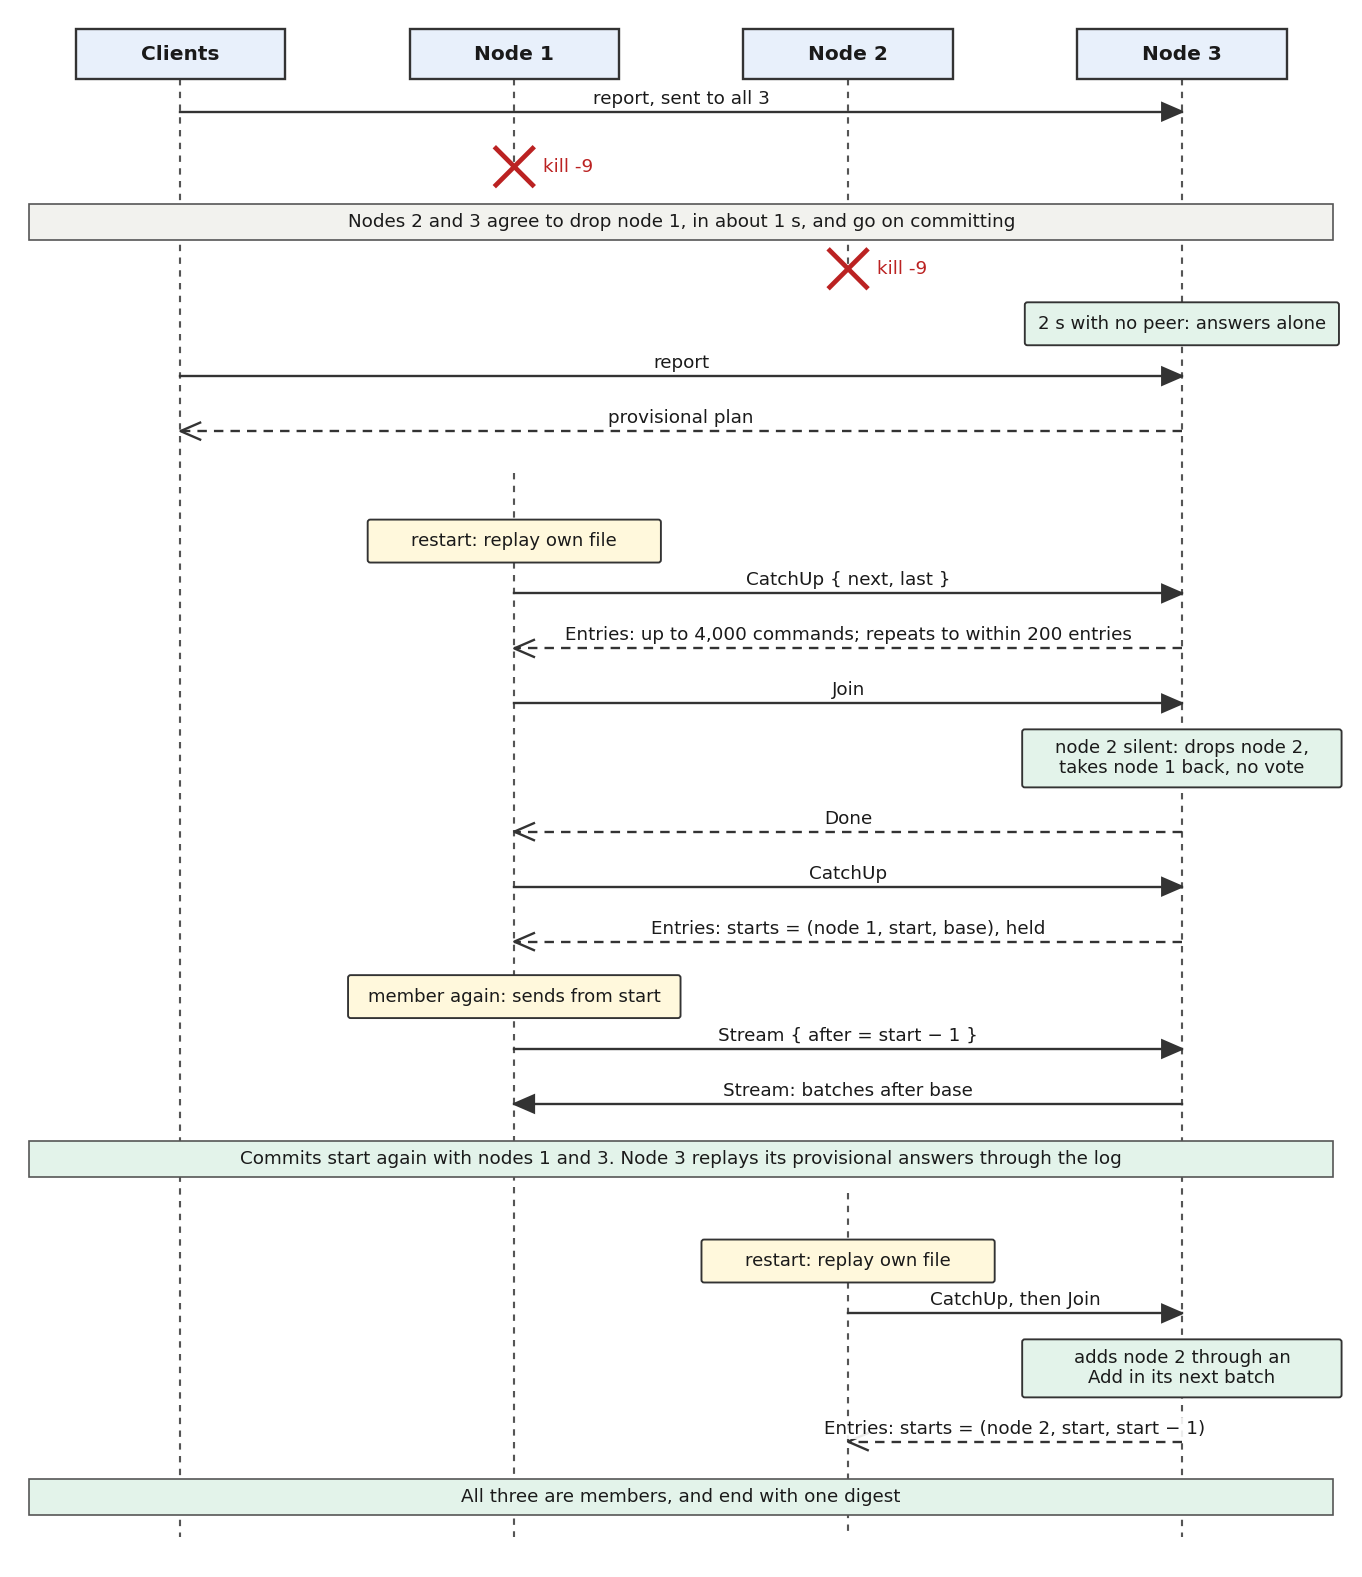
\includegraphics[width=0.84\linewidth]{figures/uml-seq-two-killed.png}
\caption{UML sequence diagram: two nodes killed, the last node answering alone, and each coming back.}
\label{fig:uml-seq-two-killed}
\end{figure}

\begin{figure}[!htb]
\centering
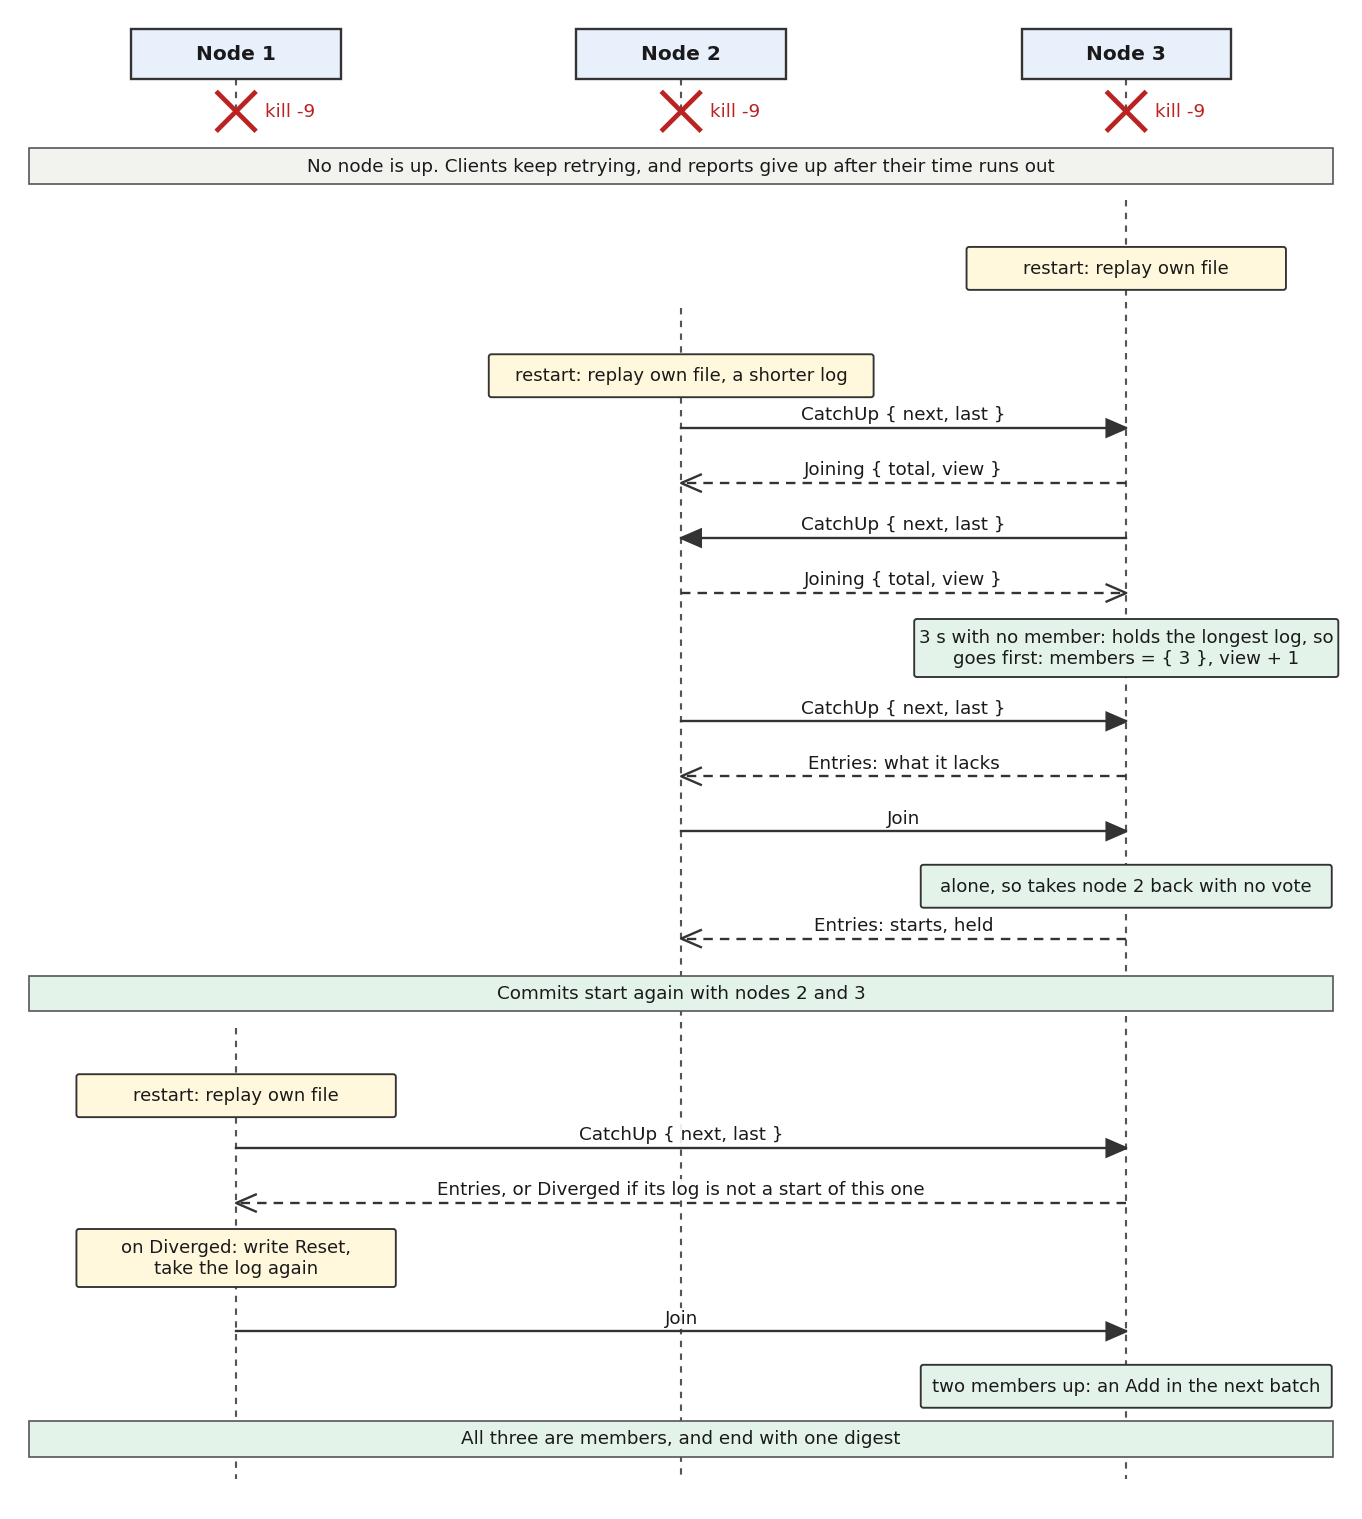
\includegraphics[width=0.84\linewidth]{figures/uml-seq-all-killed.png}
\caption{UML sequence diagram: all three nodes killed and brought back one at a time.}
\label{fig:uml-seq-all-killed}
\end{figure}

\clearpage
\subsection{State ownership}

Table~\ref{tab:ownership} says who holds each piece of state, who may change it, and whether it is shared.

\begin{table}[!htb]
\centering\small
\caption{Who owns each piece of state.}
\label{tab:ownership}
\begin{tabular}{@{}p{0.31\linewidth}p{0.14\linewidth}p{0.24\linewidth}p{0.23\linewidth}@{}}
\toprule
State & Held by & Changed by & Shared? \\
\midrule
Cloud state: results, responders, holds, digest & each node & only the state machine, in log order & the same on all nodes, through the shared log \\
Shared log: streams, waiting batches, the order applied, how far each peer has got & each node & its shared-log tasks, behind one lock & batches are copied; the counters are its own \\
Members and view of the shared log & each node & an agreed drop, an add in the log, or a lone member & agreed through those steps \\
Log file on disk & each node & one saver task & not shared; rebuilt from on restart \\
Bid rounds and planning time & each node & its own tasks & no; only the bids are sent \\
Suspicions and the group view & each node & its heartbeat task & no; each node decides for itself \\
Fault election tickets & each node & the fault election & sent to peers; not in the log \\
Worker pool queue & each node & its tasks & no \\
Provisional answers and local holds & a node left alone & degraded mode & memory only, until replayed through the log \\
Open reports, next ID, retry budget & each load program & that program's client middleware & no \\
\bottomrule
\end{tabular}
\end{table}

\subsection{Error handling}

Table~\ref{tab:errors} says what the system does when something goes wrong. A node that cannot do a job stays quiet rather than sending an error, and the client's retry covers it.

\begin{table}[!htb]
\centering\small
\caption{What happens on each error.}
\label{tab:errors}
\begin{tabular}{@{}p{0.40\linewidth}p{0.55\linewidth}@{}}
\toprule
What goes wrong & What happens \\
\midrule
No answer in the client's wait & It retries with the same ID; after 5 retries the submit call returns an error \\
A reply that rejects the report & The client does not count it as an answer, and goes on waiting \\
Worker pool full & The node logs it and sends no reply; the client's retry goes to all nodes \\
16,000 reports in progress on a node & The node refuses the report at the door, with no reply \\
A command not applied within 3 s & The proposal times out, and the node sends no reply \\
A report too old to plan & It is committed with nobody sent, and the client is told it expired \\
A peer unreachable & The call fails, the node logs it, waits a back-off, and connects again by itself \\
A log stream call fails or is not accepted yet & The sender goes back to what that peer has acknowledged, and sends again \\
A node told it is not a member & It stops serving, catches up from a member, and asks to join \\
A node's log is not a start of a member's & It writes a reset mark to its file, and takes the log again \\
A record cut short at the end of a log file & Replay stops there, and a member supplies the rest \\
A disk save fails & The node logs it \\
A damaged datagram, or a message too large for one & It is dropped and counted; the client's retry covers it \\
\bottomrule
\end{tabular}
\end{table}
